\chapter{Esperimenti e risultati}
\label{chap:esperimenti}
In questo capitolo vengono presentati i risultati ottenuti dal framework realizzato, tramite una serie di esperimenti che coinvolgono modelli e dataset differenti.\newline
Tutti gli esperimenti vengono svolti con modelli \textbf{ViT}, preaddestrati sul dataset \textbf{ImageNet}, che lavorano con \textit{patch} di dimensione \textbf{16$\times$16} e immagini in \textit{input} di tipo \textbf{RGB} con risoluzione \textbf{224$\times$224}.

\section{Dataset utilizzati}
Di seguito vengono presentati i dataset utilizzati nei test effettuati sul
framework.

\subsection{CIFAR-100}
Il primo dataset utilizzato per testare il framework è stato il
\textbf{CIFAR100}, che è stato selezionato poiché molto diffuso in letteratura,
in cui è utilizzato come \textbf{benchmark standard} per compiti di
classificazione. Risulta più complesso rispetto al \textit{CIFAR10}, ma
mantiene dimensioni ridotte e quindi permette una ottima rapidità di
\textit{training}. In particolare \textit{CIFAR100} contiene \textbf{60.000
    immagini} totali, suddivise in \textbf{50.000} immagini di addestramento e
\textbf{10.000} di validazione, tutte della risoluzione di
\textbf{32$\times$32} e di tipo \textbf{RGB}. \newline Per i test sul dataset
\textit{CIFAR100} è stata effettuata una ulteriore suddivisione del
\textit{set} di addestramento con rapporto \textbf{90/10}, in modo tale da
ottenere un \textbf{Train Set} finale di \textbf{45.000} immagini e un
\textbf{Held-Out Set} di \textbf{5.000} immagini, quest'ultimo utilizzato per
il monitoraggio del processo di compressione. \newline
\begin{figure}[H]
    \centering
    \includegraphics[width=0.8\textwidth]{images/cifar100_examples.png}
    \caption{Esempio di immagini dal dataset CIFAR100.}
    \label{fig:cifar100_examples}
\end{figure}

\subsection{ImageNet-1K}
Il secondo dataset preso in considerazione per testare il metodo è \textbf{ImageNet-1K}, utilizzatissimo in letteratura e molto più complesso rispetto al CIFAR-100. Si tratta di un \textit{benchmark} utilizzato fin dalle prime reti convoluzionali, come \textit{Alex-Net}, per valutare su task di \textit{Image Classification} e \textit{Object Detection}. Il dataset in questione risulta molto più ampio rispetto al precedente, poiché contiene circa 1.300.000 immagini di addestramento, e 50.000 immagini di validazione, tutte di tipo \textbf{RGB} ma con risoluzione variabile. \newline
Per quanto concerne i test su \textit{Imagenet-1K}, il set di addestramento è stato suddiviso con rapporto \textbf{97/3} al fine di ottenere un \textbf{Held-Out Set} di circa 38.000 immagini, per la validazione del processo di compressione ed eventuale \textit{Early Stop}. 
\begin{figure}[H]
    \centering
    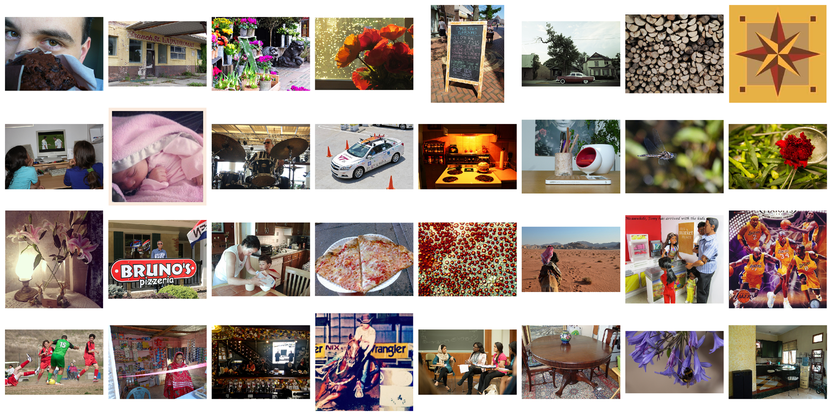
\includegraphics[width=0.9\textwidth]{images/imagenet_examples.png}
    \caption{Esempio di immagini del dataset ImageNet-1K.}
\end{figure}
\section{Data Augmentation}
Data la la grande capacità dei modelli \textit{Vision Transformer}, per
scongiurare il rischio di \textit{overfitting}, sono state adottate delle
tecniche di \textbf{Data Augmentation}, in particolare:
\begin{itemize}
    \item \textbf{Random Resized Crop}: Questa tecnica estrae una porzione casuale dell'immagine originale con un'area compresa tra l'\textbf{80\%} e il \textbf{100\%} della dimensione iniziale. Successivamente, il ritaglio viene ridimensionato alla risoluzione \textit{target} di \textbf{$224 \times 224$} pixel.
    \item \textbf{Random Horizontal Flip}: Consiste nel riflettere l'immagine orizzontalmente con una probabilità del \textbf{50\%}.
    \item \textbf{Color Jitter}: Questa trasformazione applica variazioni casuali alla luminosità, al contrasto e alla saturazione dell'immagine, con un fattore di distorsione impostato a \textbf{0.3} per ciascun parametro.
\end{itemize}
Queste sono state utilizzate per il dataset CIFAR100.

\section{Dettaglio implementativo}
\label{section:impl}
Di seguito i dettagli implementativi delle fasi di \textit{Fine Tuning} dei
modelli, durante la compressione. Per il primo \textit{Fine Tuning}:
\begin{itemize}
    \item \textbf{Ottimizzatore AdamW} con un fattore di \textbf{decadimento dei pesi} pari a \textbf{0.05} e con \textbf{learning rate discriminativi}: \textbf{$0.5 \times 10^{-5}$} per il \textit{backbone} del \textit{Transformer} e \textbf{$0.5 \times 10^{-4}$} per la testa di classificazione.
    \item \textbf{Scheduler} dei \textit{learning rate} di tipo \textbf{Cosine Annealing}.
    \item Dimensione dei \textbf{batch} di \textit{training} pari a \textbf{128}
          campioni.
    \item \textbf{30 epoche} di addestramento con \textbf{early stopping}.
\end{itemize}
Per quanto riguarda invece la fase di \textbf{Recovery Fine-Tuning}, volta a
ripristinare le prestazioni dopo il taglio dei parametri, adotta la medesima
configurazione di ottimizzazione del \textit{Fine-Tuning} iniziale, con due
variazioni: l'impiego di un \textbf{learning rate unico} pari a \textbf{$0.5
        \times 10^{-5}$} per l'intera rete e un limite massimo di \textbf{20 epoche} di
addestramento, sufficienti per stabilizzare i pesi della \textit{subnet}
individuata. \newline Infine, per quanto concerne i test con la
\textbf{Knowledge Distillation} (\textbf{KD}), è stata implementata una
versione \textit{logit-based} seguendo l'approccio proposto da \textit{Hinton
    et al.} \cite{hinton2015distilling}. Il modello \textbf{teacher}, in tutti i test, consiste nel modello \textit{ViT} che fa da \textit{Baseline}, ovvero quello integro, non sottoposto ad alcuna compressione. La funzione di
\textbf{loss composita} utilizzata durante il \textit{Recovery Fine-Tuning}
integra un termine di distillazione con temperatura \textbf{$\tau = 4.0$}. A
tale componente è stato assegnato un \textbf{peso relativo pari a $0.9$},
privilegiando così il trasferimento della conoscenza dal modello
\textit{teacher} alla \textit{subnet} compressa. Questa configurazione ha
permesso di ammorbidire le distribuzioni di probabilità dei \textit{logits},
consentendo al modello \textit{student} di apprendere non solo le etichette
corrette, ma anche le relazioni strutturali tra le classi catturate dal modello
completo. Di seguito i risultati dei test. \newline

\section{Metriche}
Per valutare le prestazioni dei modelli nei test effettuati, e di conseguenza per valutare l'efficacia del framework di compressione, sono state utilizzate le seguenti metriche:
\begin{itemize}
    \item \textbf{Numero di Parametri}: consiste nella quantità di parametri rimasti al modello, dopo l'esecuzione del processo di compressione.
    \item \textbf{Accuracy}: al fine di valutare le prestazioni del modello sul task di riferimento, viene utilizzata la \textit{Top-1 Accuracy}, valutata sui dati di test del dataset utilizzato.
    \item \textbf{GFLOPs}: si tratta del numero di \textit{Floating Point Operations} (operazioni in virgola mobile) che sono necessarie per eseguire un singolo passaggio di inferenza (\textit{forward pass}) sul modello. In particolare 1 GFLOP corrisponde ad $1 \times 10^9$ operazioni in virgola mobile. A differenza della latenza, che risulta legata all'hardware utilizzato, i GFLOPs forniscono una misura deterministica della complessità computazionale del modello.
    \item \textbf{Throughput}: consiste nel numero di immagini al secondo che vengono processate dal modello, e viene calcolato costruendo un batch di immagini "fittizie", ovvero ottenute tramite la generazione di un tensore randomico, e successivamente misurando il tempo necessario al modello per eseguire l'inferenza su tale tensore.
    \item \textbf{Latency}: viene calcolata insieme alla precedente, e misura (in ms) il tempo necessario per l'inferenza di un singolo batch di immagini.  
\end{itemize}


\section{Test sul dataset CIFAR-100}
\label{section:test}
\subsection{Test con ViT-Small}
In questi test è stato utilizzato un modello \textbf{ViT-Small} da \textbf{21.7
    Mln} di parametri, a cui è stata aggiunta una testa di classificazione da
\textbf{100 unità}, e successivamente sottoposto a \textit{Fine Tuning}
iniziale sul dataset in oggetto. Per quanto riguarda il framework, tutti i test
sono stati effettuati con \textbf{15 iterazioni} di compressione. In ogni
iterazione, la \textbf{profondità} dell'albero di ricerca è stata limitata a
\textbf{6}, questo implica che, per ogni iterazione, al modello possono essere
applicate massimo \textbf{6 azioni consecutive} di \textit{pruning}. Viene
inoltre utilizzata una \textbf{soglia di tolleranza} della fase di
\textit{Bound} pari a \textbf{0.005}, in modo tale da permettere una ricerca
più approfondita dello spazio di ricerca, al costo di un numero lievemente
maggiore di nodi esplorati. Infine, la \textbf{funzione obiettivo} utilizza un
valore di \textbf{$\lambda$} pari a \textbf{1.0}, attribuito al contributo dei
parametri. \newline 
\begin{table}[ht]
    \centering
    \label{tab:risultati-cifar100}
    \footnotesize 
    \setlength{\tabcolsep}{3pt} 
    \begin{tabular}{@{} l r r r r r @{}}
        \toprule
        \textbf{Modello} & \multicolumn{1}{c}{\textbf{Parametri (M)}} & \multicolumn{1}{c}{\textbf{Top-1 Acc. (\%)}} & \multicolumn{1}{c}{\textbf{GFLOPs}} & \multicolumn{1}{c}{\textbf{Throughput}} & \multicolumn{1}{c}{\textbf{Latency}} \\ \midrule
        Baseline           & 21.67 \hphantom{(-00.0\%)}        & 90.42\% \hphantom{(-0.00\%)}        & 4.60 \hphantom{(-00.00\%)}        & 1137.5 \hphantom{(+00.00\%)}        & 112.5 \hphantom{(-00.00\%)}       \\
        \midrule
        \textbf{Pruned}    & 15.93 (-26.6\%) & 89.59\% (-0.83\%) & 3.42 (-25.51\%) & 1405.5 (+23.56\%) & 91.1 (-19.02\%) \\
        \midrule
        \textbf{Pruned+KD} & 15.78 (-27.3\%) & 89.86\% (-0.56\%) & 3.39 (-26.19\%) & 1406.0 (+23.60\%) & 91.0 (-19.11\%) \\
        \bottomrule
    \end{tabular}
    \vspace{10pt}
    \caption{Nella tabella sono presentati i risultati comparativi utilizzando il \textit{ViT-Small} e il dataset \textit{CIFAR100}, in particolare vengono evidenziati i valori delle metriche e le variazioni rispetto al modello \textit{Baseline}.}
\end{table}

\section{Test sul dataset ImageNet-1K}
Per questi test è stato utilizzato un modello \textbf{ViT-Small} da 22 Mln di parametri. In particolare è stata aggiunta una testa di classificazione da 1000 unità, che è stata sottoposta a \textit{fine tuning} sul \textit{train set} con la \textit{backbone} del modello \textit{ViT-Small} bloccata. I parametri del framework, per tutti i test, sono stati configurati a \textbf{15 iterazioni} di compressione, la \textbf{profondità} dell'albero di ricerca è stata limitata a
\textbf{6}, la \textbf{soglia di tolleranza} della fase di
\textit{Bound} pari a \textbf{0.005}, la \textbf{funzione obiettivo} con \textbf{$\lambda$} pari a \textbf{1.0} per i parametri. \newline 
\begin{table}[ht]
    \centering
    \label{tab:risultati-cifar100}
    \footnotesize 
    \setlength{\tabcolsep}{3pt} 
    \begin{tabular}{@{} l r r r r r @{}}
        \toprule
        \textbf{Modello} & \multicolumn{1}{c}{\textbf{Parametri (M)}} & \multicolumn{1}{c}{\textbf{Top-1 Acc. (\%)}} & \multicolumn{1}{c}{\textbf{GFLOPs}} & \multicolumn{1}{c}{\textbf{Throughput}} & \multicolumn{1}{c}{\textbf{Latency}} \\ \midrule
        Baseline           & 22.05 \hphantom{(-00.0\%)}        & 81.20\% \hphantom{(-0.00\%)}        & 4.60 \hphantom{(-00.00\%)}        & 1142.6 \hphantom{(+00.00\%)}        & 112.0 \hphantom{(-00.00\%)}       \\
        \midrule
        \textbf{Pruned}    & 18.77 (-14.88\%) & 79.17\% (-2.03\%) & 3.90 (-15.13\%) & 1270.5 (+11.20\%) & 100.7 (-10.07\%) \\
        \bottomrule
    \end{tabular}
    \vspace{10pt}
    \caption{Nella tabella sono presentati i risultati comparativi utilizzando il \textit{ViT-Small} e il dataset \textit{ImageNet-1K}, in particolare vengono evidenziati i valori delle metriche e le variazioni rispetto al modello \textit{Baseline}.}
\end{table}

\section{Analisi dell'algoritmo di ricerca}
Fare test con la loss nella funzione obbiettivo, poi un altro senza la soglia
nel bound e con vari valori.

\section{Ablazione}
Al fine di verificare la bontà del metodo sono stati effettuati dei test per isolare il contributo delle due principali componenti del \textit{framework}, l'algoritmo di ricerca e la metrica di importanza. \newline
I seguenti risultati sono stati ottenuti sul dataset CIFAR100, utilizzando la stessa configurazione riportata nella sezione \ref{section:test} e nella sezione \ref{section:impl}. I test sono stati eseguiti senza l'utilizzo della \textit{Knowledge Distillation} per isolare al meglio l'effetto delle singole componenti del framework. \newline
Di seguito i risultati: \newline 
\begin{table}[ht]
    \centering
    \label{tab:risultati-ablazione}
    \footnotesize 
    \setlength{\tabcolsep}{3pt} 
    \begin{tabular}{@{} l r r r r r @{}}
        \toprule
        \textbf{Modello} & \multicolumn{1}{c}{\textbf{Parametri (M)}} & \multicolumn{1}{c}{\textbf{Top-1 Acc. (\%)}} & \multicolumn{1}{c}{\textbf{GFLOPs}} & \multicolumn{1}{c}{\textbf{Throughput}} & \multicolumn{1}{c}{\textbf{Latency}} \\ \midrule
        Baseline           & 21.67 \hphantom{(-00.0\%)}        & 90.42\% \hphantom{(-0.00\%)}        & 4.60 \hphantom{(-00.00\%)}        & 1137.5 \hphantom{(+00.00\%)}        & 112.5 \hphantom{(-00.00\%)}       \\
        \midrule
        \textbf{ViT-S Pruned (No KD)}    & 15.93 (-26.6\%) & 89.59\% (-0.83\%) & 3.43 (-25.51\%) & 1405.5 (+23.56\%) & 91.1 (-19.02\%) \\
        \midrule
        \textbf{Ricerca Disattivata} & 12.28 (-43.4\%) & 81.17\% (-9.25\%) & 2.64 (-42.66\%) & 1679.9 (+47.68\%) & 76.2 (-32.27\%) \\
        \midrule
        \textbf{Metrica Disattivata} & 19.38 (-10.7\%) & 89.07\% (-1.35\%) & 4.09 (-11.09\%) & 1147.9 (+00.09\%) & 111.5 (-00.09\%) \\
        \bottomrule
    \end{tabular}
    \vspace{10pt}
    \caption{Nella tabella sono presentati i risultati dell'applicazione del \textit{framework} di compressione nella sua interezza e con le componenti disattivate, sul dataset \textit{CIFAR100} e sul modello \textit{ViT-Small}.}
\end{table}

Come è possibile notare, entrambi i test di ablazione hanno dato risultati peggiori rispetto a quanto ottenuto con il \textit{framework} di compressione nella sua interezza. In particolare nel test con la \textbf{ricerca disattivata}, per ogni iterazione, considerando $d$ la massima profondità della ricerca, vengono eseguite casualmente $d$ azioni sul modello. In questo caso il \textit{framework} si è trovato costretto ad eseguire dei tagli su dimensioni importanti, e quindi poco conservativi dal punto di vista delle performance. La metrica di importanza, mantenuta attiva nel test, non è riuscita a limitare i danni portati dai tagli molto aggressivi e indiscriminati, portando così ad una grande diminuzione di accuratezza. Questo primo test ha dimostrato che l'algoritmo di ricerca \textit{BnB} ha un grande contributo nel selezionare accuratamente le azioni, da un lato limitando il livello di compressione a parità di iterazioni di \textit{pruning}, dall'altro consentendo di mantenere dei livelli di prestazioni molto vicini al modello originale. \newline 
Nel secondo test invece, la \textbf{metrica di importanza} è stata disattivata, di conseguenza per ogni azione selezionata dall'algoritmo di ricerca, viene prima selezionato casualmente il blocco \textit{Encoder} su cui agire, e successivamente vengono campionate casualmente le dimensioni da tagliare delle specifiche componenti (QK, MLP, \dots) di quel blocco (tranne per la dimensione di \textit{Embedding}, per il quale non è necessario selezionare prima il blocco su cui agire). I risultati indicano chiaramente una difficoltà dell'algoritmo di ricerca nell'esplorare lo spazio degli stati, causata proprio dalla mancanza dell'azione della metrica di importanza. Selezionando in maniera casuale le dimensioni da tagliare, la maggioranza degli stati (\textit{subnet}) che vengono esplorati risultano poco promettenti e peggiorano il valore della funzione obbiettivo, con un conseguente aumento del numero di nodi esplorati, ed una grande fatica a comprimere il modello. Durante i test che fanno uso della metrica di importanza, si assiste invece ad una progressione stabile e rapida del valore della funzione obbiettivo, che si dimostra quindi molto efficace nel guidare le azioni di \textit{pruning} e la ricerca. \newline 
In questo secondo test è importante notare come le prestazioni del modello si sono mantenute elevate, a conferma del grande lavoro di filtraggio eseguito dal processo di ricerca, che evita di selezionare quegli stati, la cui selezione casuale dei tagli, ha danneggiato gravemente il modello. 


